\subsection{热平衡}
设将$A$和$B$两个相封闭在一个与环境隔绝(与环境无热量和物质的交换)的体系内,$A$与$B$两相之间只有热量交换,即$A,B$两相间的隔板完全固定,只能导热。如图1.1所示,设此时从$A$有微量的热传到$B$内,则$A,B$两相的内能变化为
\begin{equation}
\begin{aligned}
\mathrm{d}U_A-T_AdS_A-P_AdV_A, \\
\mathrm{d}U_B-T_BdS_B-P_AdV_B
\end{aligned}
\end{equation}
由于隔板固定,故$A,B$两相的体积也固定,故$dV_A=dV_B=0$。
\begin{figure}[h]
 \centering
 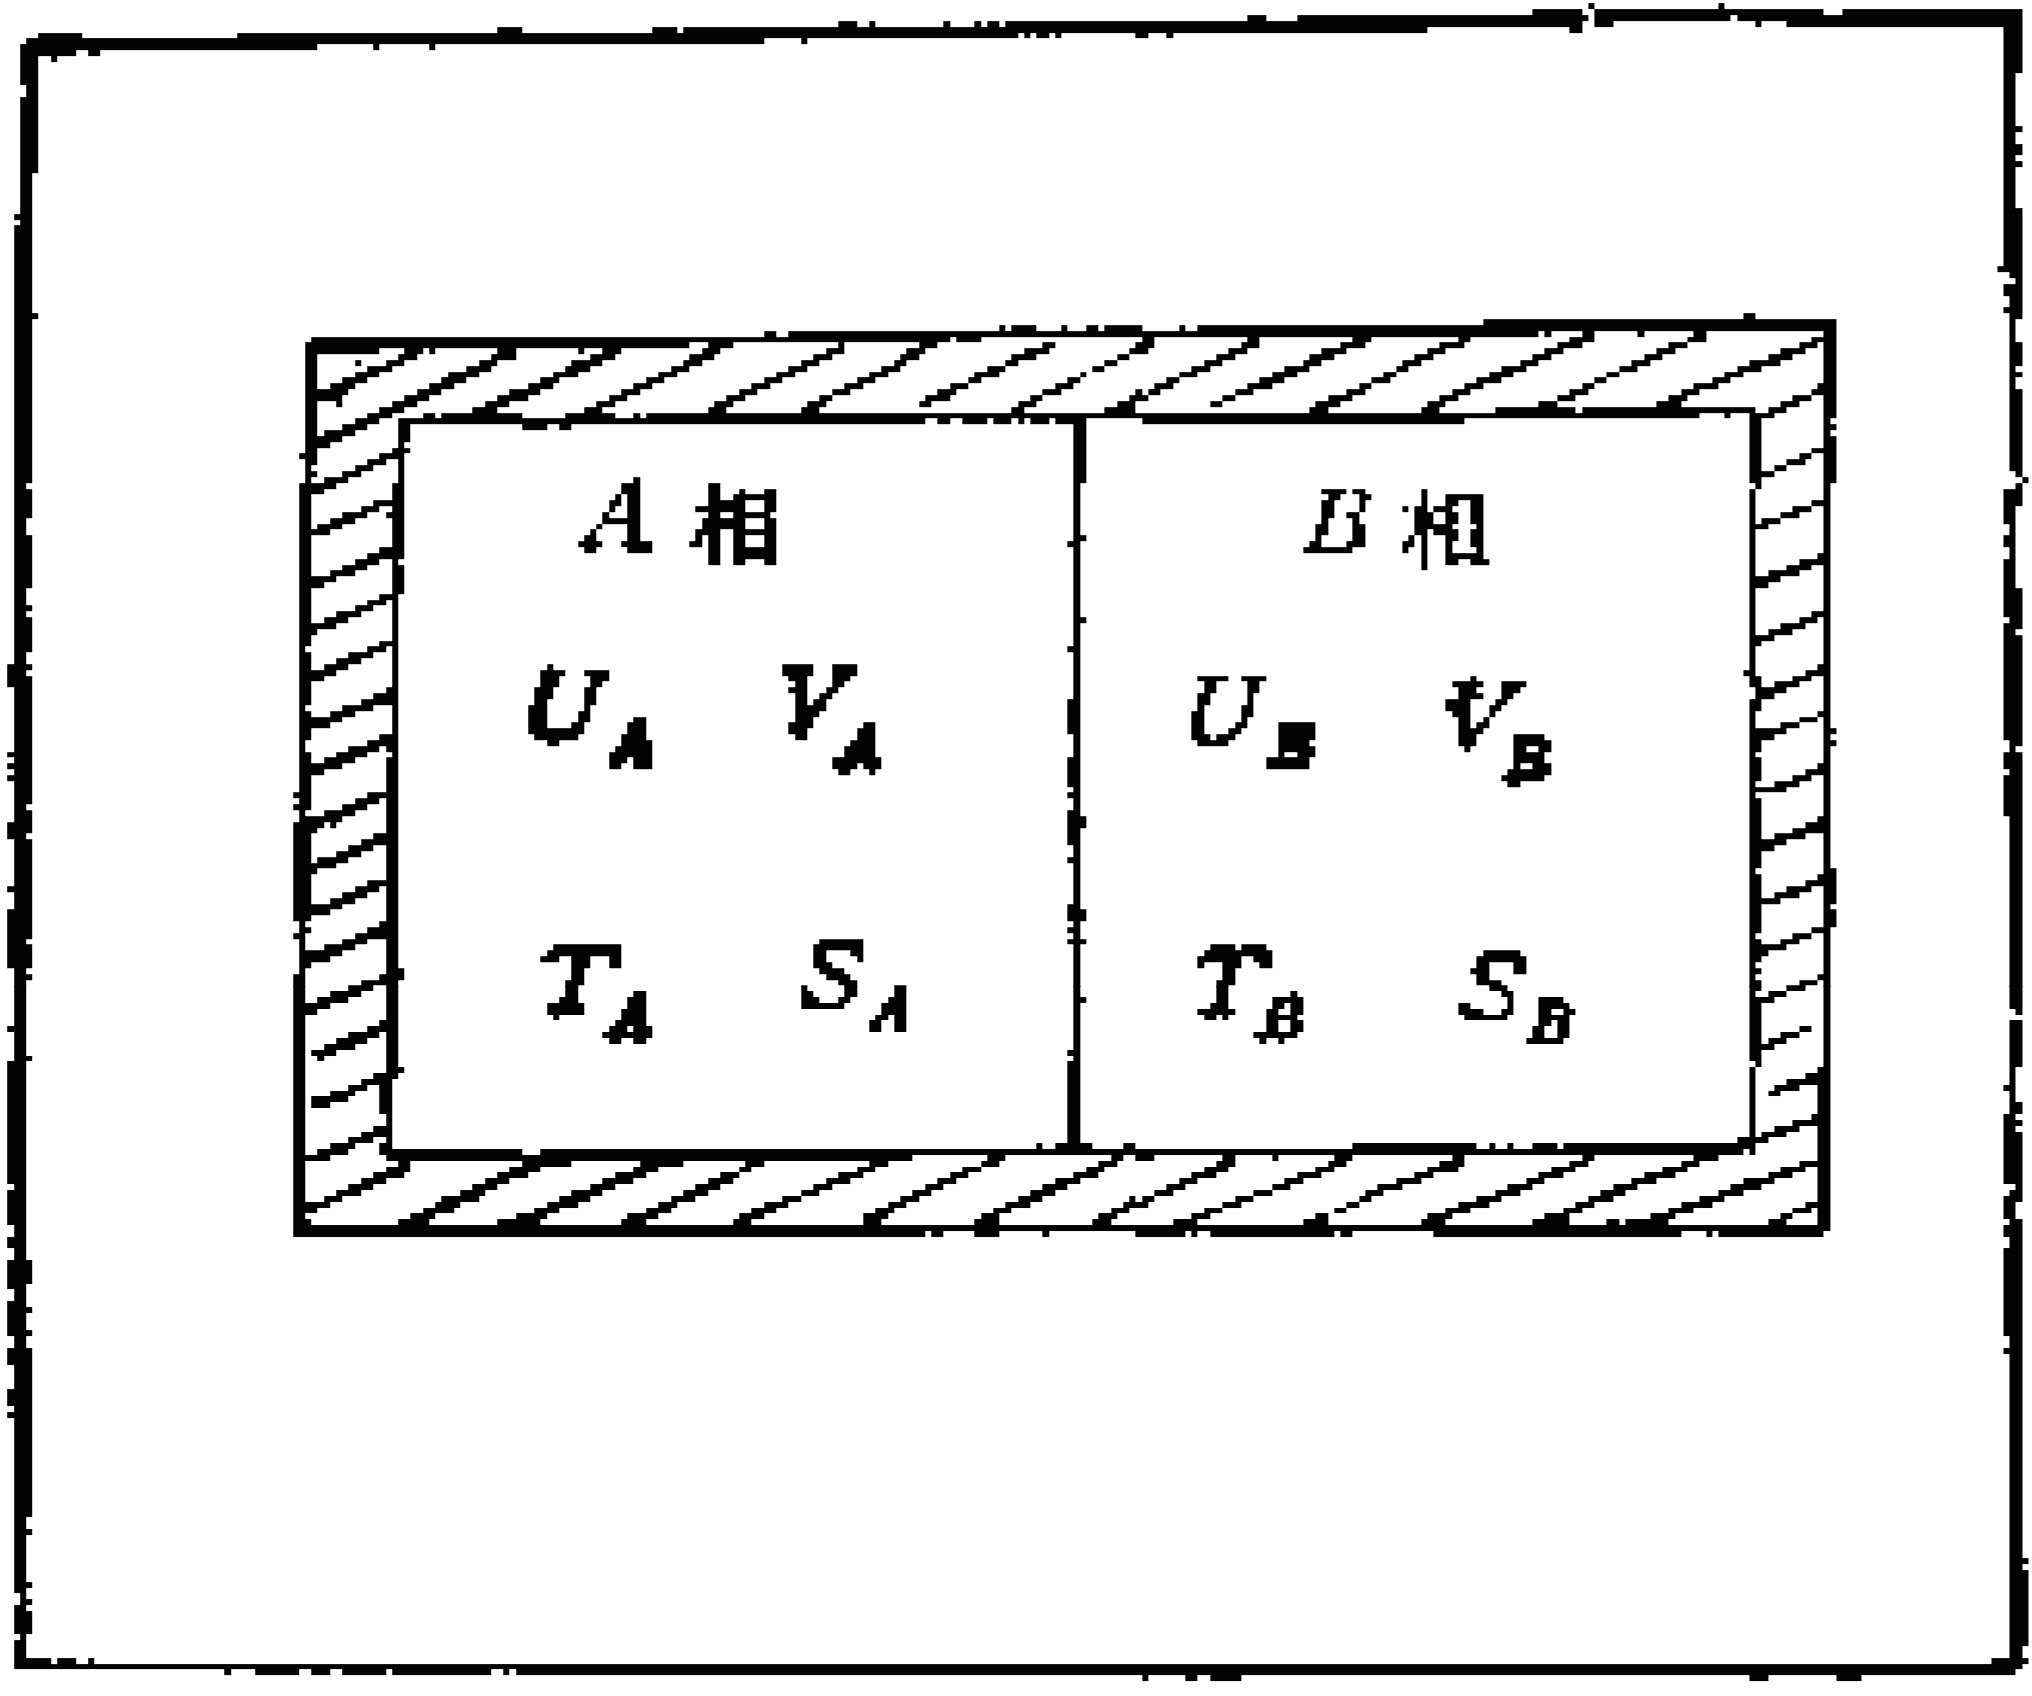
\includegraphics[width=0.4\textwidth]{fig/cp01/img1.1.jpg}
 \caption{推导两相间热平衡所用示意图。}
\end{figure}
这说明此时体系内能的变化只表现为热的改变,即
$$\delta Q=-dU_A=dU_B.$$
这里假定由$A$传至$B$时,对$B$相来说,$\delta Q$为正,反方向为负。于是式(1.1)可写为
\begin{equation}
-\delta Q/T_A=dS_A,\ \ \delta Q/T_B=dS_B.
\end{equation}
两式相加,得
$$\frac{\delta Q(T_A-T_B)}{T_AT_B}=dS_A+dS_B=d(S_A+S_B)\geq 0$$
不平衡时,$d(S_A+S_B)>0$,即$T_A>T_B$,热量由高温传至低温。当体系处于平衡态时,熵应为最大,也即$d(S_A+S_B)=0$,于是得出$\delta Q(T_A-T_B)=0$,但$\delta Q\neq 0$,故有
\begin{equation}T_A=T_B\end{equation}
这就是说,两相在互相接触的情况下达到平衡时,温度应该相等。